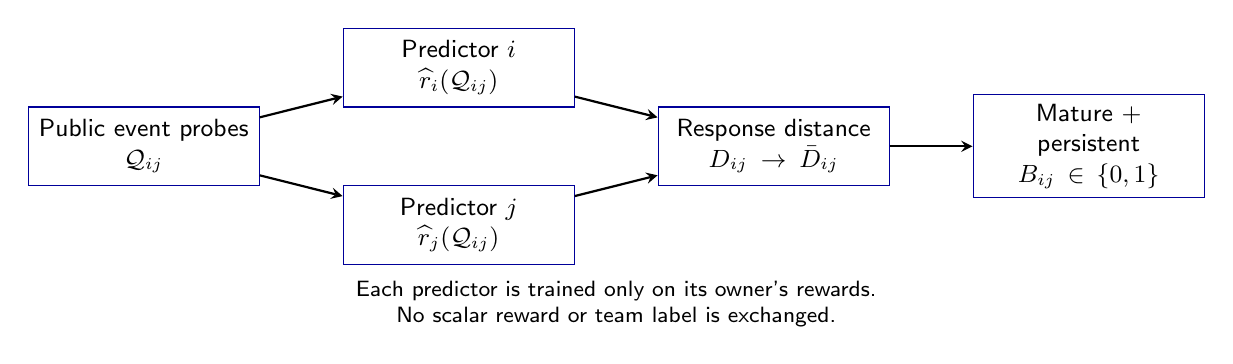
\begin{tikzpicture}[font=\sffamily\small,>=stealth,b/.style={draw=blue!60!black,align=center,text width=27mm,minimum height=10mm},a/.style={->,thick}]
\node[b] (q) at (0,0) {Public event probes\\$\mathcal Q_{ij}$};
\node[b] (i) at (4,1) {Predictor $i$\\$\widehat r_i(\mathcal Q_{ij})$};
\node[b] (j) at (4,-1) {Predictor $j$\\$\widehat r_j(\mathcal Q_{ij})$};
\node[b] (dist) at (8,0) {Response distance\\$D_{ij}\to\bar D_{ij}$};
\node[b] (b) at (12,0) {Mature + persistent\\$B_{ij}\in\{0,1\}$};
\draw[a](q)--(i);\draw[a](q)--(j);\draw[a](i)--(dist);\draw[a](j)--(dist);\draw[a](dist)--(b);
\node[font=\sffamily\footnotesize,align=center] at (6,-2) {Each predictor is trained only on its owner's rewards.\\ No scalar reward or team label is exchanged.};
\end{tikzpicture}
